\subsection{Cuprates: High temperature superconductors}
\begin{figure}
    \centering
    \begin{subfigure}{0.37\textwidth}
        \centering
        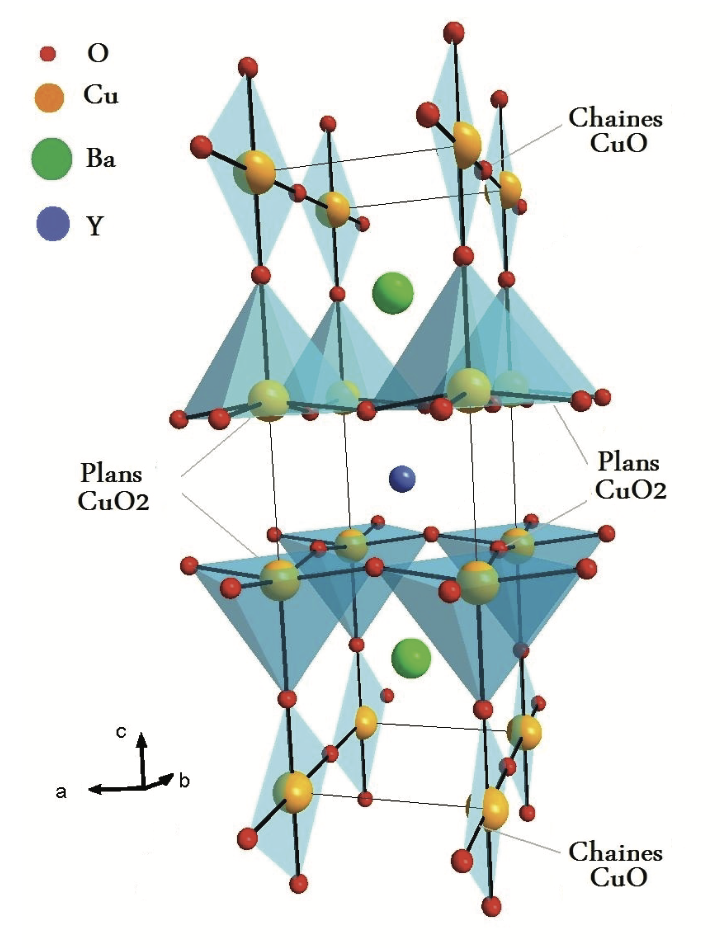
\includegraphics[width=\textwidth]{figures/cuprate_structure}
        \caption{Crystal structure of a Cuprate (YBCO)}
        \label{fig:cuprate_structure}
    \end{subfigure}\hfill
    \begin{subfigure}{0.5\textwidth}
        \centering
        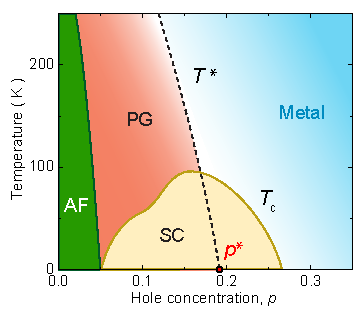
\includegraphics[width=\textwidth]{figures/phase_diagram}
        \caption{Phase diagram of cuprates}
        \label{fig:phase_diagram}
    \end{subfigure}
    \caption{Physical description of cuprates. (a) shows the perovskite structure of a cuprate,
    and (b) shows the different phases of cuprates in a phase diagram. $p^*$ marks the hypothesised
    quantum critical point. AF, PG, and SC stand for Antiferromagnetic, Pseudogap, and
    Superconducting phases respectively.}
\end{figure}

Cuprates are a class of superconductors with high critical temperature that have been subject
to intense research since their discovery in 1986 because the origin of their superconductivity is not well understood. They have a general formula $XYCu_mO_n$ (where $X$ and $Y$ can be a variety of elements) and exhibit rich physical behavior, 
with a diverse phase diagram.

The crystal structure of cuprates is a perovskite structure, with a copper-oxygen plane
($\mathrm{CuO}_2$) as the main conducting layer. This structure is shown in Figure
\ref{fig:cuprate_structure}. You can think of cuprates as a stack of different conducting layers,
so the electronic properties of cuprates are mainly 2D. However, the interlayer coupling is
non-negligible, and the 3D nature of cuprates is important for their physical properties.

The phase diagram of cuprates is shown in Figure \ref{fig:phase_diagram}. The main phases of
cuprates are the antiferromagnetic (AF) phase, the metallic phase, the pseudogap (PG) phase,
the superconducting (SC) phase. 
The metallic phase itself can be split into a strange metal phase 
(with anomalous electronic scattering properties) and a normal metal phase 
(with well-described conductivity, using Fermi liquid theory).
The pseudogap phase is one of the most intriguing phases in the phase diagram, 
with many peculiarities (such as no real phase transition with the metallic phase), 
the details of which are beyond the scope of our project.
There is also a hypothesised point in the phase diagram called the quantum critical point, marked as $p^*$ in the figure.
